\pagebreak
\thispagestyle{empty}
\movetoevenpage
\begin{figure}
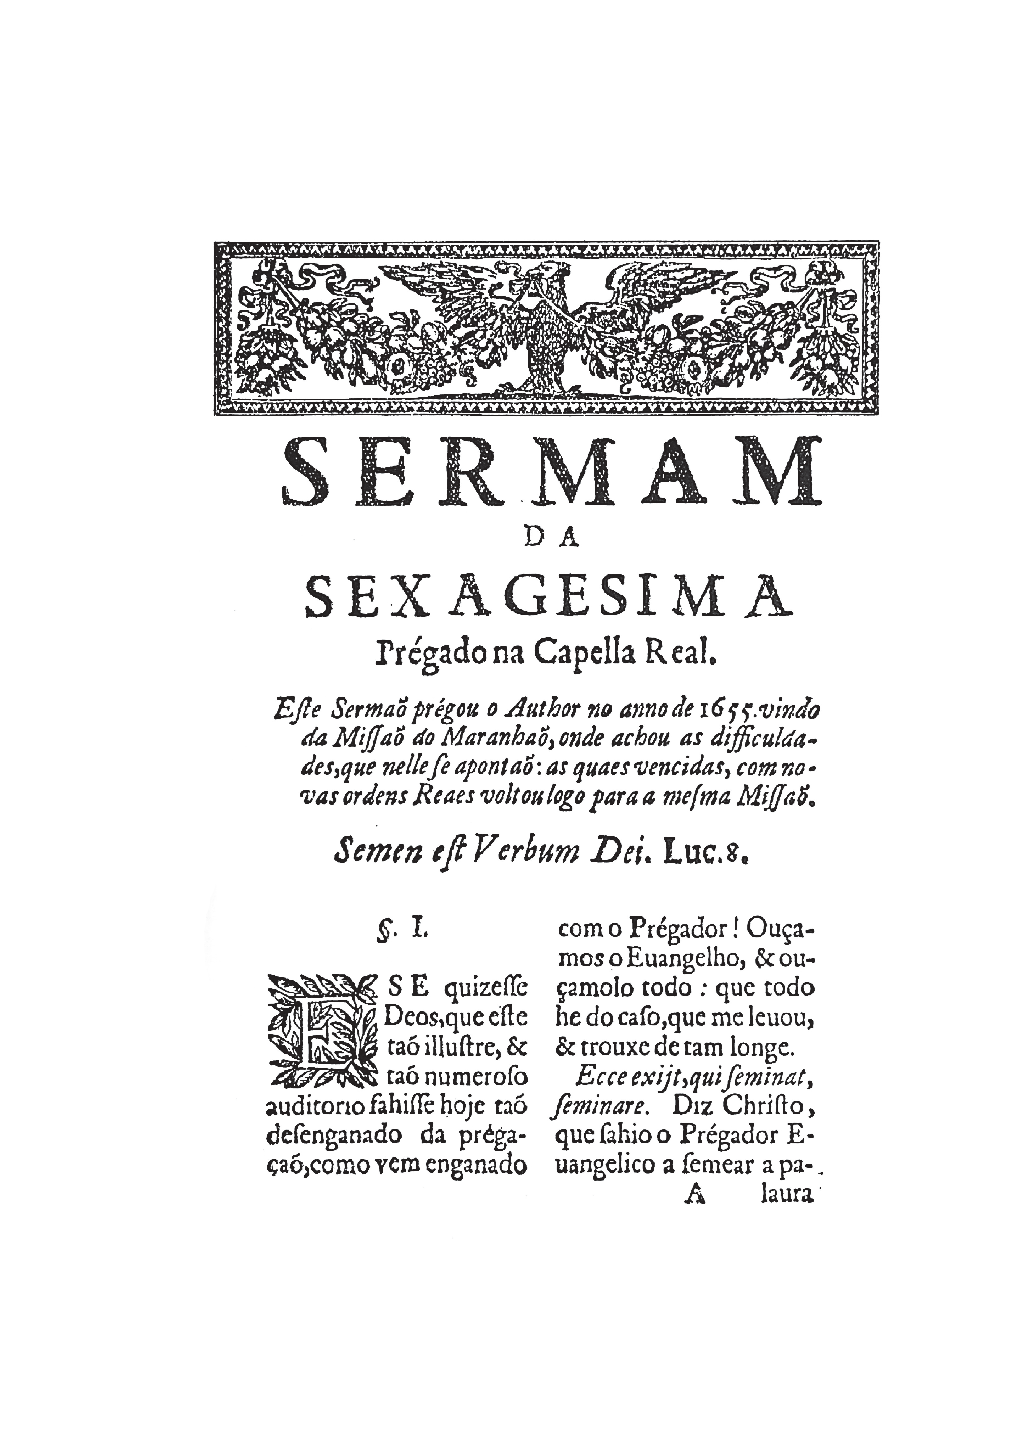
\includegraphics[width=\textwidth]{./imgs/sexagesima.pdf}  
\end{figure}

\chapter{Sermão da Sexagésima}


\begin{quotation}
\noindent\textbf{Pregado na Capela Real}\\
Este Sermão pregou o Autor no ano 1655 vindo da Missão do Maranhão,
onde achou as dificuldades que nele se apontam: as quais vencidas, com novas ordens Reais voltou logo para a mesma Missão
\end{quotation}


\epigraph{\textit{Semen est verbum Dei.}}{ S.\,Lucas, \textsc{viii}, 11.}

\section{i}

\noindent{}E se quisesse Deus que este tão ilustre e tão numeroso auditório saísse
hoje tão desenganado da pregação, como vem enganado com o pregador!
Ouçamos o Evangelho, e ouçamo"-lo todo, que todo é do caso que me levou e
trouxe de tão longe.

\emph{Ecce exiit qui seminat, seminare}. Diz Cristo que saiu o pregador evangélico a semear a palavra divina. Bem parece este texto dos
livros de Deus. Não só faz menção do semear, mas também faz caso do
sair: \emph{Exiit}, porque no dia da messe hão"-nos de medir a semeadura
e hão"-nos de contar os passos. O Mundo, aos que lavrais com ele, nem vos
satisfaz o que dispendeis, nem vos paga o que andais. Deus não é assim.
Para quem lavra com Deus até
o sair é semear, porque também das passadas colhe fruto. Entre os
semeadores do Evangelho há uns que saem a semear, há outros que
semeiam sem sair. Os que saem a semear são os que vão pregar à Índia, à
China, ao Japão; os que semeiam sem sair, são os que se contentam com
pregar na Pátria. Todos terão sua razão, mas tudo tem sua conta. Aos que
têm a seara em casa, pagar"-lhes"-ão a semeadura; aos que vão buscar a
seara tão longe, hão"-lhes de medir a semeadura e hão"-lhes de contar os
passos. Ah Dia do Juízo! Ah pregadores! Os de cá, achar"-vos"-eis com mais
paço; os de lá, com mais passos: \emph{Exiit seminare.}


Mas daqui mesmo vejo que notais (e me notais) que diz Cristo que o
semeador do Evangelho saiu, porém não diz que tornou porque os
pregadores evangélicos, os homens que professam pregar e propagar a Fé,
é bem que saiam, mas não é bem que tornem. Aqueles animais de Ezequiel
que tiravam pelo carro triunfal da glória de Deus e significavam os
pregadores do Evangelho, que propriedades tinham? \emph{Nec
revertebantur, cum ambularent}: Uma vez que iam, não tornavam. As
rédeas por que se governavam era o ímpeto do espírito, como diz o mesmo
texto; mas esse espírito tinha impulsos para os levar, não tinha
regresso para os trazer; porque sair para tornar, melhor é não sair.
Assim arguís com muita razão, e eu também assim o digo. Mas pergunto: E
se esse semeador evangélico, quando saiu, achasse o campo tomado; se se
armassem contra ele os espinhos; se se levantassem contra ele as pedras,
e se lhe fechassem os caminhos, que havia de fazer? Todos estes
contrários que digo e todas estas contradições experimentou o semeador
do nosso Evangelho. Começou ele a semear (diz Cristo), mas com pouca
ventura. Uma parte do trigo caiu entre espinhos, e afogaram"-no os
espinhos: \emph{Aliud cecidit inter spinas, et simul exortae spinae
suffocaverunt illud}. Outra parte caiu sobre pedras, e secou"-se nas
pedras por falta de humidade: \emph{Aliud cecidit super petram, et
natum aruit, quia non habebat humorem.} Outra parte caiu no caminho,
e pisaram"-no os homens e comeram"-no as aves: \emph{Aliud cecidit secus
viam, et conculcatum est, et volucres coeli comederunt illud.} Ora vede
como todas as criaturas do Mundo se armaram contra esta sementeira.
Todas as criaturas quantas há no Mundo se reduzem a quatro géneros: criaturas racionais, como os homens; criaturas sensitivas, como os animais;
criaturas vegetativas, como as plantas; criaturas insensíveis, como as
pedras; e não há mais. Faltou alguma destas que se não armasse contra o
semeador? Nenhuma. A natureza insensível o perseguiu nas pedras, a
vegetativa nos espinhos, a sensitiva nas aves, a racional nos homens.
E notai a desgraça do trigo, que onde só podia esperar razão, ali achou
maior agravo. As pedras secaram"-no, os espinhos afogaram"-no, as aves
comeram"-no; e os homens? Pisaram"-no: \emph{Conculcatum est}. (\emph{Ab
hominibus}, diz a Glossa).
Quando Cristo mandou pregar os Apóstolos pelo Mundo, disse"-lhes desta
maneira: \emph{Euntes in mundum universum, praedicate omni creaturae}:
Ide, e pregai a toda a criatura. Como assim, Senhor?! Os animais não
são criaturas?! As árvores não são criaturas?! As pedras não são
criaturas?! Pois hão os Apóstolos de pregar às pedras?! Hão"-de pregar
aos troncos?! Hão"-de pregar aos animais?! Sim, diz S.\,Gregório, depois
de Santo Agostinho. Porque como os Apóstolos iam pregar a todas as
nações do Mundo, muitas delas bárbaras e incultas, haviam de achar os
homens degenerados em todas as espécies de criaturas: haviam de achar
homens homens, haviam de achar homens brutos, haviam de achar homens
troncos, haviam de achar homens pedras. E quando os pregadores evangélicos vão pregar a toda a criatura, que se armem contra eles todas as
criaturas?! Grande desgraça!

Mas ainda a do semeador do nosso Evangelho não foi a maior. A maior é a
que se tem experimentado na seara aonde eu fui, e para onde venho. Tudo
o que aqui padeceu o trigo, padeceram lá os semeadores. Se bem
advertirdes, houve aqui trigo mirrado, trigo afogado, trigo comido e
trigo pisado. Trigo mirrado: \emph{Natum aruit, quia non habebat
humorem}; trigo afogado: \emph{Exortae spinae suffocaverunt illud};
trigo comido: \emph{Volucres caeli comederunt illud}; trigo pisado:
\emph{Conculcatum est}. Tudo isto padeceram os semeadores evangélicos
da missão do Maranhão de doze anos a esta parte. Houve missionários
afogados, porque uns se afogaram na boca do grande rio das Amazonas;
houve missionários comidos, porque a outros comeram os bárbaros na ilha
dos Aroãs; houve missionários mirrados, porque tais tornaram os da
jornada dos Tocantins, mirrados da fome e da doença, onde tal houve, que
andando vinte e dois dias perdido nas brenhas matou somente a sede com o
orvalho que lambia das folhas. Vede se lhe quadra bem o \emph{Natum
aruit, quia non habebat humorem!} E que sobre mirrados, sobre
afogados, sobre comidos, ainda se vejam pisados e perseguidos dos
homens: \emph{Conculcatum est!} Não me queixo nem o digo, Senhor, pelos
semeadores; só pela seara o digo, só pela seara o sinto. Para os
semeadores, isto são glórias: mirrados sim, mas por amor de vós
mirrados; afogados sim, mas por amor de vós
afogados; comidos sim, mas por amor de vós comidos; pisados e
perseguidos sim, mas por amor de vós perseguidos e pisados.

Agora torna a minha pergunta: E que faria neste caso, ou que devia fazer
o semeador evangélico, vendo tão mal logrados seus primeiros trabalhos?
Deixaria a lavoura? Desistiria da sementeira? Ficar"-se"-ia ocioso no
campo, só porque tinha lá ido? Parece que não. Mas se tornasse muito
depressa a buscar alguns instrumentos com que alimpar a terra das
pedras e dos espinhos, seria isto desistir? Seria isto tornar atrás?
Não por certo. No mesmo texto de Ezequiel com que arguistes, temos a
prova. Já vimos como dizia o texto, que aqueles animais da carroça de
Deus, quando iam não tornavam: \emph{Nec revertebantur, cum
ambularent.} Lede agora dois versos mais abaixo, e vereis que diz o
mesmo texto que aqueles animais tornavam, e semelhança de um raio ou
corisco: \emph{Ibant et revertebantur in similitudinem fulguris
coruscantis.} Pois se os animais iam e tornavam à semelhança de um raio,
como diz o texto que quando iam não tornavam? Porque quem vai e volta
como um raio, não torna. Ir e voltar como raio, não é tornar, é ir por
diante. Assim o fez o semeador do nosso Evangelho. Não o desanimou nem a
primeira nem a segunda nem a terceira perda; continuou por diante no
semear, e foi com tanta felicidade, que nesta quarta e última parte do
trigo se restauraram com vantagem as perdas do demais: nasceu,
cresceu, espigou, amadureceu, colheu"-se, mediu"-se, achou"-se que por um
grão multiplicara cento: \emph{Et fecit fructum centuplum.}

Oh que grandes esperanças me dá esta sementeira! Oh que
grande exemplo me dá este semeador! Dá"-me grandes esperanças a
sementeira, porque, ainda que se perderam os primeiros trabalhos,
lograr"-se"-ão os últimos. Dá"-me grande exemplo o semeador, porque, depois
de perder a primeira, a segunda e a terceira parte do trigo, aproveitou
a quarta e última, e colheu dela muito fruto. Já que se perderam as três
partes da vida, já que uma parte da idade a levaram os espinhos, já que
outra parte a levaram as pedras, já que outra parte a levaram os
caminhos, e tantos caminhos, esta quarta e última parte, este último
quartel da vida, porque se perderá também? Porque não dará fruto?
Porque não terão também os anos o que tem o ano? O ano tem tempo para as
flores e tempo para os
frutos. Porque não terá também o seu Outono a vida? As flores, umas
caem, outras secam, outras murcham, outras leva o vento; aquelas poucas
que se pegam ao tronco e se convertem em fruto, só essas são as
venturosas, só essas são as que aproveitam, só essas são as que
sustentam o Mundo. Será bem que o Mundo morra à fome? Será bem que os
últimos dias se passem em flores? Não será bem, nem Deus quer que
seja, nem há"-de ser. Eis aqui porque eu dizia ao princípio, que vindes
enganados com o pregador. Mas para que possais ir desenganados com o
sermão, tratarei nele uma matéria de grande peso e importância. Servirá
como de prólogo aos sermões que vos hei"-de pregar, e aos mais que
ouvirdes esta Quaresma.

\section{II\break\textit{Semen est verbum Dei}}


O trigo que semeou o pregador evangélico, diz Cristo que é a palavra
de Deus. Os espinhos, as pedras, o caminho e a terra boa em que o trigo
caiu, são os diversos corações dos homens. Os espinhos são os corações
embaraçados com cuidados, com riquezas, com delícias; e nestes
afoga"-se a palavra de Deus. As pedras são os corações duros e
obstinados; e nestes seca"-se a palavra de Deus, e se nasce, não cria
raízes. Os caminhos são os corações inquietos e perturbados com a
passagem e tropel das coisas do Mundo, umas que vão, outras que vêm,
outras que atravessam, e todas passam; e nestes é pisada a palavra de
Deus, porque a desatendem ou a desprezam. Finalmente, a terra boa são
os corações bons ou os homens de bom coração; e nestes prende e
frutifica a palavra divina, com tanta fecundidade e abundância, que se
colhe cento por um: \emph{Et fructum fecit centuplum.}

Este grande frutificar da palavra de Deus é o em que reparo hoje; e é
uma dúvida ou admiração que me traz suspenso e confuso, depois que
subo ao púlpito. Se a palavra de Deus é tão eficaz e tão poderosa, como
vemos tão pouco fruto da palavra de Deus? Diz Cristo que a palavra de
Deus frutifica cento por um, e já eu me contentara com que frutificasse
um por cento. Se com cada cem sermões se convertera e emendara um homem,
já o Mundo fora santo. Este argumento de fé, fundado na autoridade de
Cristo, se
aperta ainda mais na experiência, comparando os tempos passados com os
presentes. Lede as histórias eclesiásticas, e achá"-las"-eis todas cheias
de admiráveis efeitos da pregação da palavra de Deus. Tantos pecadores
convertidos, tanta mudança de vida, tanta reformação de costumes; os
grandes desprezando as riquezas e vaidades do Mundo; os reis renunciando
os ceptros e as coroas; as mocidades e as gentilezas metendo"-se pelos
desertos e pelas covas; e hoje? Nada disto. Nunca na Igreja de Deus
houve tantas pregações, nem tantos pregadores como hoje. Pois se tanto
se semeia a palavra de Deus, como é tão pouco o fruto? Não há um homem
que em um sermão entre em si e se resolva, não há um moço que se
arrependa, não há um velho que se desengane. Que é isto? Assim como Deus
não é hoje menos omnipotente, assim a sua palavra não é hoje menos
poderosa do que dantes era. Pois se a palavra de Deus é tão poderosa; se
a palavra de Deus tem hoje tantos pregadores, porque não vemos hoje
nenhum fruto da palavra de Deus? Esta, tão grande e tão importante
dúvida, será a matéria do sermão. Quero começar pregando"-me a mim. A mim
será, e também a vós; a mim, para aprender a pregar; a vós, que
aprendais a ouvir.

\section{III}

Fazer pouco fruto a palavra de Deus no Mundo, pode proceder de um de
três princípios: ou da parte do pregador, ou da parte do ouvinte, ou da
parte de Deus. Para uma alma se converter por meio de um sermão, há"-de
haver três concursos: há"-de concorrer o pregador com a doutrina,
persuadindo; há"-de concorrer o ouvinte com o entendimento, percebendo;
há"-de concorrer Deus com a graça, alumiando. Para um homem se ver a si
mesmo, são necessárias três coisas: olhos, espelho e luz. Se tem
espelho e é cego, não se pode ver por falta de olhos; se tem espelho e
olhos, e é de noite, não se pode ver por falta de luz. Logo, há mister
luz, há mister espelho e há mister olhos. Que coisa é a conversão de uma
alma, senão entrar um homem dentro em si e ver"-se a si mesmo? Para esta
vista são necessários olhos, e necessária luz e é necessário espelho.
O pregador concorre com o espelho, que é a doutrina; Deus concorre com a
luz, que é a graça; o homem concorre com
os olhos, que é o conhecimento. Ora suposto que a conversão das almas
por meio da pregação depende destes três concursos: de Deus, do pregador
e do ouvinte, por qual deles devemos entender que falta? Por parte do
ouvinte, ou por parte do pregador, ou por parte de Deus?

Primeiramente, por parte de Deus, não falta nem pode faltar. Esta
proposição é de fé, definida no Concílio Tridentino, e no nosso
Evangelho a temos. Do trigo que deitou à terra o semeador, uma parte se
logrou e três se perderam. E porque se perderam estas três? A
primeira perdeu"-se, porque a afogaram os espinhos; a segunda, porque a
secaram as pedras; a terceira, porque a pisaram os homens e a comeram
as aves. Isto é o que diz Cristo; mas notai o que não diz. Não diz que
parte alguma daquele trigo se perdesse por causa do sol ou da chuva. A
causa por que ordinariamente se perdem as sementeiras, é pela
desigualdade e pela intemperança dos tempos, ou porque falta ou sobeja a
chuva, ou porque falta ou sobeja o sol. Pois porque não introduz Cristo
na parábola do Evangelho algum trigo que se perdesse por causa do sol ou
da chuva? Porque o sol e a chuva são as influências da parte do Céu,
e deixar de frutificar a semente da palavra de Deus, nunca é por falta
do Céu, sempre é por culpa nossa. Deixará de frutificar a sementeira, ou
pelo embaraço dos espinhos, ou pela dureza das pedras, ou pelos
descaminhos dos caminhos; mas por falta das influências do Céu, isso
nunca é nem pode ser. Sempre Deus está pronto da sua parte, com o sol
para aquentar e com a chuva para regar; com o sol para alumiar e com a
chuva para amolecer, se os nossos corações quiserem: \emph{Qui solem
suum oriri facit super bonos et malos, et pluit super justos et
injustos.} Se Deus dá o seu sol e a sua chuva aos
bons e aos maus; aos maus que se quiserem fazer bons, como a negará?
Este ponto é tão claro que não há para que nos determos em mais prova.
\emph{Quid debui facere vineae meae, et non feci?}
disse o mesmo Deus por Isaías.

Sendo, pois, certo que a palavra divina não deixa de frutificar
por parte de Deus, segue"-se que ou é por falta do pregador ou por
falta dos ouvintes. Por qual será? Os pregadores deitam a culpa aos
ouvintes, mas não é assim. Se fora por parte dos ouvintes, não fizera a
palavra de Deus muito grande fruto, mas não fazer nenhum fruto e
nenhum efeito, não é por parte dos ouvintes. Provo. Os ouvintes, ou são
maus ou são bons; se são bons, faz neles fruto a palavra de Deus; se são maus, ainda que não faça neles
fruto, faz efeito. No Evangelho o temos. O trigo que caiu nos espinhos,
nasceu, mas afogaram"-no: \emph{Simul exortae spinae suffocaverunt
illud.} O trigo que caiu nas pedras, nasceu também, mas secou"-se:
\emph{Et natum aruit.} O trigo que caiu na terra boa, nasceu e
frutificou com grande multiplicação: \emph{Et natum fecit fructum centuplum.} De maneira que o trigo que caiu na boa terra, nasceu e
frutificou; o trigo que caiu na má terra, não frutificou, mas nasceu;
porque a palavra de Deus é tão fecunda, que nos bons faz muito fruto e é
tão eficaz que nos maus, ainda que não faça fruto, faz efeito; lançada
nos espinhos, não frutificou, mas nasceu até nos espinhos; lançada nas
pedras, não frutificou, mas nasceu até nas pedras. Os piores ouvintes
que há na Igreja de Deus, são as pedras e os espinhos. E porquê? Os
espinhos por agudos, as pedras por duras. Ouvintes de entendimentos
agudos e ouvintes de vontades endurecidas são os piores que há. Os
ouvintes de entendimentos agudos são maus ouvintes, porque vêm só a
ouvir subtilezas, a esperar galantarias, a avaliar pensamentos, e às
vezes também a picar a quem os não pica. \emph{Aliud cecidit inter
spinas:} O trigo não picou os espinhos, antes os espinhos o picaram a
ele; e o mesmo sucede cá. Cuidais que o sermão vos picou a vós, e não é
assim; vós sois os que picais o sermão. Por isto são maus ouvintes os de
entendimentos agudos. Mas os de vontades endurecidas ainda são piores,
porque um entendimento agudo pode ferir pelos mesmos fios, e vencer"-se
uma agudeza com outra maior; mas contra vontades endurecidas nenhuma
coisa aproveita a agudeza, antes dana mais, porque quanto as setas são
mais agudas, tanto mais facilmente se despontam na pedra. Oh! Deus nos
livre de vontades endurecidas, que ainda são piores que as pedras! A
vara de Moisés abrandou as pedras, e não pôde abrandar uma vontade
endurecida:
\emph{Percutiens virga bis silicem, et egressae sunt aquae
largissimae}. \emph{Induratum est cor
Pharaonis}. E com os ouvintes de entendimentos
agudos e os ouvintes de vontades endurecidas serem os mais rebeldes, é
tanta a força da divina palavra, que, apesar da agudeza, nasce nos
espinhos, e apesar da dureza nasce nas pedras.
Pudéramos arguir ao lavrador do Evangelho de não cortar os espinhos e de
não arrancar as pedras antes de semear, mas de indústria deixou no
campo as pedras e os espinhos, para que se visse a força do que semeava.
É tanta a força da divina palavra, que, sem cortar nem despontar
espinhos, nasce entre espinhos. É tanta a força da divina palavra, que,
sem arrancar nem abrandar pedras, nasce nas pedras. Corações embaraçados
como espinhos, corações secos e duros como pedras, ouvi a palavra de
Deus e tende confiança! Tomai exemplo nessas mesmas pedras e nesses
espinhos! Esses espinhos e essas pedras agora resistem ao semeador do
Céu; mas virá tempo em que essas mesmas pedras o aclamem e esses mesmos
espinhos o coroem.
Quando o semeador do Céu deixou o campo, saindo deste Mundo, as pedras
se quebraram para lhe fazerem aclamações, e os espinhos se teceram para
lhe fazerem coroa. E se a palavra de Deus até dos espinhos e das pedras
triunfa; se a palavra de Deus até nas pedras, até nos espinhos nasce;
não triunfar dos alvedrios hoje a palavra de Deus, nem nascer nos
corações, não é por culpa, nem por indisposição dos ouvintes.

Supostas estas duas demonstrações; suposto que o fruto e efeitos da
palavra de Deus, não fica, nem por parte de Deus, nem por parte dos
ouvintes, segue"-se por consequência clara, que fica por parte do
pregador. E assim é. Sabeis, cristãos, porque não faz fruto a palavra de
Deus? Por culpa dos pregadores. Sabeis, pregadores, porque não faz
fruto a palavra de Deus? Por culpa nossa.

\section{IV}

Mas como em um pregador há tantas qualidades, e em uma pregação tantas
leis, e os pregadores podem ser culpados em todas,
em qual consistirá esta culpa? No pregador podem"-se considerar
cinco circunstâncias: a pessoa, a ciência, a matéria, o estilo, a voz. A
pessoa que é, a ciência que tem, a matéria que trata, o estilo que
segue, a voz com que fala. Todas estas circunstâncias temos no
Evangelho. Vamo"-las examinando uma por uma e buscando esta causa.

Será porventura o não fazer fruto hoje a palavra de Deus, pela
circunstância da pessoa? Será porque antigamente os pregadores eram
santos, eram varões apostólicos e exemplares, e hoje os pregadores são
eu e outros como eu? Boa razão é esta. A definição do pregador é a
vida e o exemplo. Por isso Cristo no Evangelho não o comparou ao
semeador, senão ao que semeia. Reparai. Não diz Cristo: saiu a semear o
\emph{semeador}, senão, saiu a semear \emph{o que semeia}: \emph{Ecce
exiit, qui seminat, seminare.} Entre o semeador e o que semeia há muita
diferença. Uma coisa é o soldado e outra coisa o que peleja; uma coisa é
o governador e outra o que governa. Da mesma maneira, uma coisa é o
semeador e outra o que semeia; uma coisa é o pregador e outra o que
prega. O semeador e o pregador é nome; o que semeia e o que prega é
acção; e as acções são as que dão o ser ao pregador. Ter o nome de
pregador, ou ser pregador de nome, não importa nada; as acções, a vida,
o exemplo, as obras, são as que convertem o Mundo. O melhor conceito
que o pregador leva ao púlpito, qual cuidais que é? É o conceito que
de sua vida têm os ouvintes.
Antigamente convertia"-se o Mundo, hoje porque se não converte ninguém? Porque hoje pregam"-se palavras e pensamentos, antigamente
pregavam"-se palavras e obras. Palavras sem obra são tiros sem bala;
atroam, mas não ferem. A funda de David derrubou o gigante, mas não o
derrubou com o estalo, senão com a pedra: \emph{Infixus est lapis in
fronte ejus.} As vozes da harpa de David lançavam
fora os demónios do corpo de Saul, mas não eram vozes pronunciadas com a
boca, eram vozes formadas com a mão: \emph{David tollebat citharam, et
percutiebat manu sua.} Por isso Cristo comparou o
pregador ao semeador. O pregar que é falar, faz"-se com a boca; o pregar
que é semear, faz"-se com a mão. Para falar
ao vento, bastam palavras; para falar ao coração, são necessárias obras.
Diz o Evangelho que a palavra de Deus frutificou cento por um. Que quer
isto dizer? Quer dizer que de uma palavra nasceram cem palavras? Não.
Quer dizer que de poucas palavras nasceram muitas obras. Pois palavras
que frutificam obras, vede se podem ser só palavras! Quis Deus converter
o Mundo, e que fez? Mandou ao Mundo seu Filho feito homem. Notai. O
Filho de Deus, enquanto Deus, é palavra de Deus, não é obra de Deus:
\emph{Genitum, non factum}. O Filho de Deus, enquanto Deus e Homem, é
palavra de Deus e obra de Deus juntamente: \emph{Verbum caro factum
est.} De maneira que até de sua palavra desacompanhada de obras não fiou
Deus a conversão dos homens. Na união da palavra de Deus com a maior
obra de Deus consistiu a eficácia da salvação do Mundo. Verbo Divino é
palavra divina; mas importa pouco que as nossas palavras sejam divinas,
se forem desacompanhadas de obras. A razão disto é porque as palavras
ouvem"-se, as obras vêem"-se; as palavras entram pelos ouvidos, as obras
entram pelos olhos, e a nossa alma rende"-se muito mais pelos olhos que
pelos ouvidos. No Céu ninguém há que não ame a Deus, nem possa deixar de
o amar. Na terra há tão poucos que o amem, todos o ofendem. Deus não é o
mesmo, e tão digno de ser amado no Céu e na Terra? Pois como no Céu
obriga e necessita a todos a o amarem, e na terra não? A razão é porque
Deus no Céu é Deus visto; Deus na terra é Deus ouvido. No Céu entra o
conhecimento de Deus à alma pelos olhos: \emph{Videbimus eum sicut est};
na terra entra"-lhe o conhecimento de Deus pelos ouvidos: \emph{Fides ex
auditu}; e o que entra pelos ouvidos crê"-se, o que entra pelos olhos
necessita. Viram os ouvintes em nós o que nos ouvem a nós, e o abalo e
os efeitos do sermão seriam muito outros.

Vai um pregador pregando a Paixão, chega ao pretório de Pilatos, conta como a Cristo o fizeram rei de zombaria, diz que tomaram
uma púrpura e lha puseram aos ombros; ouve aquilo o auditório muito
atento. Diz que teceram uma coroa de espinhos e que lha pregaram na
cabeça; ouvem todos com a mesma atenção. Diz mais que lhe ataram as
mãos e lhe meteram nelas uma cana por ceptro; continua o mesmo silêncio
e a mesma suspensão nos ouvintes. Corre"-se neste espaço uma cortina,
aparece a imagem do \emph{Ecce Homo}; eis todos prostrados por terra, eis todos a
bater no peito, eis as lágrimas, eis os gritos, eis os alaridos, eis as
bofetadas. Que é isto? Que apareceu de novo nesta igreja? Tudo o que
descobriu aquela cortina, tinha já dito o pregador. Já tinha dito
daquela púrpura, já tinha dito daquela coroa e daqueles espinhos, já
tinha dito daquele ceptro e daquela cana. Pois se isto então não fez
abalo nenhum, como faz agora tanto? Porque então era \emph{Ecce
Homo} ouvido, e agora é \emph{Ecce Homo} visto; a relação do pregador
entrava pelos ouvidos a representação daquela figura entra pelos olhos.
Sabem, Padres pregadores, porque fazem pouco abalo os nossos sermões? Porque não pregamos aos olhos, pregamos só aos ouvidos. Porque
convertia o Baptista tantos pecadores? Porque assim como as suas
palavras pregavam aos ouvidos, o seu exemplo pregava aos olhos. As
palavras do Baptista pregavam penitência: \emph{Agite poenitentiam.}
Homens, fazei penitência, e o exemplo clamava: \emph{Ecce Homo}: eis, aqui está o homem que
é o retrato da penitência e da aspereza. As palavras do Baptista
pregavam jejum e repreendiam os regalos e demasias da gula; e o exemplo
clamava: \emph{Ecce Homo}: eis aqui está o homem que se sustenta de
gafanhotos e mel silvestre. As palavras do Baptista pregavam composição
e modéstia, e condenavam a soberba e a vaidade das galas; e o exemplo
clamava: \emph{Ecce Homo}: eis aqui está o homem vestido de peles de
camelo, com as cordas e cilício à raiz da carne. As palavras do Baptista
pregavam despegos e retiros do Mundo, e fugir das ocasiões e dos
homens; e o exemplo clamava: \emph{Ecce Homo}: eis aqui o homem que
deixou as cortes e as sociedades, e vive num deserto e numa cova. Se os
ouvintes ouvem uma coisa e vêem outra, como se hão"-de converter? Jacob
punha as varas manchadas diante das ovelhas quando concebiam, e daqui
procedia que os cordeiros nasciam manchados. Se quando os ouvintes
percebem os nossos conceitos, têm diante dos olhos as nossas manchas,
como hão"-de conceber virtudes? Se a minha vida é apologia contra a minha
doutrina, se as minhas palavras vão já refutadas nas minhas obras, se
uma coisa é o semeador e outra o que semeia, como se há"-de fazer fruto?

Muito boa e muito forte razão era esta de não fazer fruto a
palavra de Deus; mas tem contra si o exemplo e experiência de
Jonas. Jonas fugitivo de Deus, desobediente, contumaz, e, ainda depois
de engolido e vomitado, iracundo, impaciente, pouco caritativo, pouco
misericordioso, e mais zeloso e amigo da própria estimação que da honra
de Deus e salvação das almas, desejoso de ver subvertida a Nínive e de a
ver subverter com seus olhos, havendo nela tantos mil inocentes; contudo
este mesmo homem com um sermão converteu o maior rei, a maior corte e o
maior reinado do Mundo, e não de homens fiéis senão de gentios idólatras. Outra é logo a causa que buscamos. Qual será?

\section{V}

Será porventura o estilo que hoje se usa nos púlpitos? Um estilo tão
empeçado, um estilo tão dificultoso, um estilo tão afectado, um estilo
tão encontrado a toda a arte e a toda a natureza? Boa razão é também
esta. O estilo há"-de ser muito fácil e muito natural. Por isso Cristo
comparou o pregar ao semear: \emph{Exiit, qui seminat, seminare.}
Compara Cristo o pregar ao semear, porque o semear é uma arte que tem
mais de natureza que de arte. Nas outras artes tudo é arte: na música
tudo se faz por compasso, na arquitectura tudo se faz por regra, na
aritmética tudo se faz por conta, na geometria tudo se faz por medida.
O semear não é assim. É uma arte sem arte, caia onde cair. Vede como
semeava o nosso lavrador do Evangelho. Caía o trigo nos espinhos e
nascia: \emph{Aliud cecidit inter spinas, et simul exortae spinae}.
Caía o trigo nas pedras e nascia: \emph{Aliud cecidit super petram,
et ortum.} Caía o trigo na terra boa e nascia: \emph{Aliud cecidit
in terram bonam, et natum.} Ia o trigo caindo e ia nascendo.

Assim há"-de ser o pregar. Hão"-de cair as coisas e hão"-de nascer; tão
naturais que vão caindo, tão próprias que venham nascendo. Que
diferente é o estilo violento e tirânico que hoje se usa! Ver vir os
tristes passos da Escritura, como quem vem ao martírio; uns vêm
acarretados, outros vêm arrastados, outros vêm estirados, outros vêm
torcidos, outros vêm despedaçados; só atados não vêm! Há tal tirania?
Então no meio disto, que bem levantado está aquilo! Não está a coisa no
levantar, está no cair: \emph{Cecidit.} Notai uma alegoria própria da
nossa língua. O trigo do semeador, ainda
que caiu quatro vezes, só de três nasceu; para o sermão vir nascendo,
há"-de ter três modos de cair: há"-de cair com queda, há"-de cair com
cadência, há"-de cair com caso. A queda é para as coisas, a cadência para
as palavras, o caso para a disposição. A queda é para as coisas, porque
hão"-de vir bem trazidas e em seu lugar; hão"-de ter queda. A cadência é
para as palavras, porque não hão"-de ser escabrosas nem dissonantes;
hão"-de ter cadência. O caso é para a disposição, porque há"-de ser tão
natural e tão desafectada que pareça caso e não estudo: \emph{Cecidit,
cecidit, cecidit.}

Já que falo contra os estilos modernos, quero alegar por mim o estilo do
mais antigo pregador que houve no Mundo. E qual foi ele? O mais
antigo pregador que houve no Mundo foi o céu. \emph{Coeli enarrant
gloriam Dei et opera manuum ejus annuntiat Firmamentum}, diz David.
Suposto que o céu é pregador, deve de ter sermões e deve de ter:
palavras. Sim, tem, diz o mesmo David; tem palavras e tem sermões; e
mais, muito bem ouvidos. \emph{Non sunt loquellae, nec sermones, quorum
non audiantur voces eorum.} E quais são estes sermões e estas palavras
do céu? As palavras são as estrelas, os sermões são a composição, a
ordem, a harmonia e o curso delas. Vede como diz o estilo de pregar do
céu, com o estilo que Cristo ensinou na terra. Um e outro é semear; a
terra semeada de trigo, o céu semeado de estrelas. O pregar há"-de ser
como quem semeia, e não como quem ladrilha ou azuleja. Ordenado, mas
como as estrelas: \emph{Stellae manentes in ordine suo.} Todas as
estrelas estão por sua ordem; mas é ordem que faz influência, não é
ordem que faça lavor. Não fez Deus o céu em xadrez de estrelas, como os
pregadores fazem o sermão em xadrez de palavras. Se de uma parte há"-de
estar \emph{branco}, da outra há"-de estar \emph{negro}; se de uma parte
dizem \emph{luz}, da outra hão"-de dizer \emph{sombra}; se de uma parte
dizem \emph{desceu}, da outra hão"-de dizer \emph{subiu}. Basta que não
havemos de ver num sermão duas palavras em paz? Todas hão"-de estar
sempre em fronteira com o seu contrário? Aprendamos do céu o estilo da
disposição, e também o das palavras. As estrelas são muito distintas e
muito claras. Assim há"-de ser o estilo da pregação; muito distinto e
muito claro. E nem por isso temais que pareça o estilo baixo; as
estrelas são muito distintas e muito claras, e altíssimas. O estilo pode
ser muito claro e muito alto;
tão claro que o entendam os que não sabem e tão alto que tenham muito
que entender os que sabem. O rústico acha documentos nas estrelas para
sua lavoura e o mareante para sua navegação e o matemático para as suas
observações e para os seus juízos. De maneira que o rústico e o
mareante, que não sabem ler nem escrever, entendem as estrelas; e o
matemático, que tem lido quantos escreveram, não alcança a entender
quanto nelas há. Tal pode ser o sermão: estrelas que todos vêem, e
muito poucos as medem.

Sim, Padre; porém esse estilo de pregar não é pregar culto. Mas fosse!
Este desventurado estilo que hoje se usa, os que o querem honrar
chamam"-lhe \emph{culto}, os que o condenam chamam"-lhe \emph{escuro},
mas ainda lhe fazem muita honra. O estilo culto não é escuro, é negro, e
negro boçal e muito cerrado. E possível que somos portugueses e
havemos de ouvir um pregador em português e não havemos de entender o
que diz?! Assim como há Lexicon para o grego e Calepino para o latim,
assim é necessário haver um vocabulário do púlpito. Eu ao menos o tomara
para os nomes próprios, porque os cultos têm desbaptizados os santos,
e cada autor que alegam é um enigma. Assim o disse o \emph{Ceptro
Penitente}, assim o disse o \emph{Evangelista Apeles}, assim o disse a
\emph{Águia de África}, o \emph{Favo de Claraval}, a \emph{Púrpura de
Belém}, a \emph{Boca de Ouro}. Há tal modo de alegar! O \emph{Ceptro
Penitente} dizem que é David, como se todos os ceptros não foram
penitência; o \emph{Evangelista Apeles}, que é S.\,Lucas; o \emph{Favo de
Claraval}, S.\,Bernardo; a \emph{Águia de África}, Santo Agostinho; a
\emph{Púrpura de Belém}, S.\,Jerónimo; a \emph{Boca de Ouro}, S.\,Crisóstomo. E quem quitaria ao outro cuidar que a \emph{Púrpura de
Belém} é Herodes, que a \emph{Águia de África} é Cipião, e que a
\emph{Boca de Ouro} é Midas? Se houvesse um advogado que alegasse assim
a Bártolo e Baldo, havíeis de fiar dele o vosso pleito? Se houvesse um
homem que assim falasse na conversação, não o havíeis de ter por
néscio? Pois o que na conversação seria necedade, como há"-de ser
discrição no púlpito?

Boa me parecia também esta razão; mas como os cultos pelo
pulido e estudado se defendem com o grande Nazianzeno, com Ambrósio, com
Crisólogo, com Leão, e pelo escuro e duro, com Clemente Alexandrino, com
Tertuliano, com Basílio de Selêucia, com Zeno Veronense e outros, não
podemos negar a reverência a
tamanhos autores, posto que desejáramos, nos que se prezam de beber
destes rios, a sua profundidade. Qual será logo a causa de nossa queixa?

\section{VI}

Será pela matéria ou matérias que tomam os pregadores? Usa"-se hoje o
modo que chamam de apostilar o Evangelho, em que tomam muitas matérias,
levantam muitos assuntos e quem levanta muita caça e não segue nenhuma
não é muito que se recolha com as mãos vazias. Boa razão é também esta.
O sermão há"-de ter um só assunto e uma só matéria. Por isso Cristo disse
que o lavrador do Evangelho não semeara muitos géneros de sementes,
senão uma só: \emph{Exiit, qui seminat, seminare semen}. Semeou uma
semente só, e não muitas, porque o sermão há"-de ter uma só matéria, e
não muitas matérias. Se o lavrador semeara primeiro trigo, e sobre o
trigo semeara centeio, e sobre o centeio semeara milho grosso e miúdo, e
sobre o milho semeara cevada, que havia de nascer? Uma mata brava,
uma confusão verde. Eis aqui o que acontece aos sermões deste género.
Como semeiam tanta variedade, não podem colher coisa certa. Quem semeia
misturas, mal pode colher trigo. Se uma nau fizesse um bordo para o
norte, outro para o sul, outro para leste, outro para oeste, como
poderia fazer viagem? Por isso nos púlpitos se trabalha tanto e se
navega tão pouco. Um assunto vai para um vento, outro assunto vai para
outro vento; que se há"-de colher senão vento? O Baptista convertia
muitos em Judeia; mas quantas matérias tomava? Uma só matéria:
\emph{Parate viam Domini;} a preparação para o Reino de Cristo. Jonas
converteu os Ninivitas; mas quantos assuntos tomou? Um só assunto:
\emph{Adhuc quadraginta dies, et Ninive subvertetur}: a subversão da
cidade. De maneira que Jonas em quarenta dias pregou um só assunto; e
nós queremos pregar quarenta assuntos em uma hora! Por isso não pregamos
nenhum. O sermão há"-de ser de uma só cor, há"-de ter um só objecto, um só
assunto, uma só matéria.

Há"-de tomar o pregador uma só matéria, há"-de defini"-la para
que se conheça, há"-de dividi"-la para que se distinga, há"-de prová"-la
com a Escritura, há"-de declará"-la com a razão, há"-de confirmá"-la com o
exemplo, há"-de amplificá"-la com as causas, com os efeitos, com as circunstâncias, com as conveniências que se hão"-de seguir,
com os inconvenientes que se devem evitar, há"-de responder às dúvidas,
há"-de satisfazer às dificuldades, há"-de impugnar e refutar com toda a
força da eloquência os argumentos contrários, e depois disto há"-de
colher, há"-de apertar, há"-de concluir, há"-de persuadir, há"-de acabar.
Isto é sermão, isto é pregar; e o que não é isto, é falar de mais alto.
Não nego nem quero dizer que o sermão não haja de ter variedade de
discursos, mas esses hão"-de nascer todos da mesma matéria e continuar e
acabar nela. Quereis ver tudo isto com os olhos? Ora vede: Uma árvore
tem raízes, tem tronco, tem ramos, tem folhas, tem varas, tem flores,
tem frutos. Assim há"-de ser o sermão: há"-de ter raízes fortes e sólidas,
porque há"-de ser fundado no Evangelho; há"-de ter um tronco, porque
há"-de ter um só assunto e tratar uma só matéria; deste tronco hão"-de
nascer diversos ramos, que são diversos discursos, mas nascidos da
mesma matéria e continuados nela; estes ramos não hão"-de ser secos, senão cobertos de folhas, porque os discursos hão"-de ser vestidos e
ornados de palavras. Há"-de ter esta árvore varas, que são a repreensão
dos vícios; há"-de ter flores, que são as sentenças; e por remate de tudo
isto, há"-de ter frutos, que é o fruto e o fim a que se há"-de ordenar o
sermão. De maneira que há"-de haver frutos, há"-de haver flores, há"-de
haver varas, há"-de haver folhas, há"-de haver ramos, mas tudo nascido e
fundado em um só tronco, que é uma só matéria. Se tudo são troncos, não
é sermão, é madeira. Se tudo são ramos, não é sermão, são maravalhas. Se
tudo são folhas, não é sermão, são verças. Se tudo são varas, não é
sermão, é feixe. Se tudo são flores, não é sermão, é ramalhete. Serem
tudo frutos, não pode ser; porque não há frutos sem árvore. Assim que
nesta árvore, à que podemos chamar \emph{árvore da vida}, há"-de haver o
proveitoso do fruto, o formoso das flores, o rigoroso das varas,
o vestido das folhas, o estendido dos ramos; mas tudo isto
nascido e formado de um só tronco, e esse não levantado no ar, senão
fundado nas raízes do Evangelho: \emph{Seminare semen}. Eis aqui como
hão"-de ser os sermões, eis aqui como não são. E assim não é muito que se
não faça frutos com eles.

Tudo o que tenho dito pudera demonstrar largamente, não só com os
preceitos dos Aristóteles, dos Túlios, dos Quintilianos, mas com a
prática observada do príncipe dos oradores evangélicos: S.\,João
Crisóstomo, S.\,Basílio Magno, S.\,Bernardo. S.\,Cipriano, e com as
famosíssimas orações de S.\,Gregório Nazianzeno, mestre de ambas as
Igrejas. E posto que nestes mesmos Padres, como em Santo Agostinho, S.\,Gregório e muitos outros, se acham os Evangelhos apostilados com nomes
de sermão e homilias, uma coisa é expor, e outra pregar; uma ensinar e
outra persuadir. E desta última é que eu falo, com a qual tanto fruto
fizeram no Mundo Santo António de Pádua e S.\,Vicente Ferrer. Mas nem por
isso entendo que seja ainda esta a verdadeira causa que busco.

\section{VII}

Será porventura a falta de ciência que há em muitos pregadores? Muitos
pregadores há que vivem do que não colheram e semeiam o que não
trabalharam. Depois da sentença de Adão, a terra não costuma dar fruto,
senão a quem come o seu pão com o suor do seu rosto. Boa razão parece
também esta. O pregador há"-de pregar o seu e não o alheio. Por isso diz
Cristo que semeou o lavrador do Evangelho o trigo seu: \emph{Semen
suum.} Semeou o seu e não o alheio, porque o alheio e o furtado não é
bom para semear, ainda que o furto seja de ciência. Comeu Eva o pomo da
ciência, e queixava"-me eu antigamente desta nossa mãe; já que comeu o
pomo, por que lhe não guardou as pevides? Não seria bem que chegasse a
nós a árvore, já que nos chegaram os encargos dela? Pois porque não o
fez assim Eva? Porque o pomo era furtado, e o alheio é bom para
comer, não é bom para semear: é bom para comer, porque dizem que é
saboroso; não é bom para semear, porque não nasce. Alguém terá
experimentado que o alheio lhe nasce em casa, mas esteja certo, que se
nasce, não há"-de deitar raízes, e o que não tem raízes não pode dar
fruto. Eis aqui por que muitos pregadores não fazem fruto; porque pregam
o alheio, e não o seu: \emph{semen suum.} O pregar é entrar em batalha
com os vícios; e armas alheias, ainda que sejam as de Aquiles, a ninguém
deram vitória. Quando David saiu a campo com o gigante, ofereceu"-lhe
Saul as suas armas, mas ele não as quis aceitar. Com as armas alheias ninguém
pode vencer, ainda que seja David. As armas de Saul só servem a Saul, e
as de David a David; e mais aproveita um cajado e uma funda própria, que
a espada e a lança alheia. Pregador que peleja com as armas alheias, não
hajais medo que derribe gigante.

Fez Cristo aos Apóstolos pescadores de homens, que foi ordená"-los de
pregadores; e que faziam os Apóstolos? Diz o texto que estavam
\emph{reficientes retia sua}: refazendo as redes suas; eram as redes
dos Apóstolos, e não eram alheias. Notai: \emph{retia sua}. Não diz que
eram suas porque as compraram, senão que eram suas porque as faziam; não
eram suas porque lhes custaram o seu dinheiro, senão porque lhes
custavam o seu trabalho. Desta maneira eram as redes suas; e porque
desta maneira eram suas, por isso eram redes de pescadores que haviam de
pescar homens. Com redes alheias ou feitas por mãos alheias, podem"-se
pescar peixes, homens não se podem pescar. A razão disto é porque nesta
pesca de entendimentos só quem sabe fazer a rede sabe fazer o lanço.
Como se faz uma rede? Do fio e do nó se compõe a malha; quem não
enfia nem ata, como há"-de fazer rede? E quem não sabe enfiar nem sabe
atar, como há"-de pescar homens? A rede tem chumbada que vai ao fundo, e
tem cortiça que nada em cima da água. A pregação tem umas coisas de mais
peso e de mais fundo, e tem outras mais superficiais e mais leves; e
governar o leve e o pesado, só o sabe fazer quem faz a rede. Na boca de
quem não faz a pregação, até o chumbo é cortiça.
As razões não hão"-de ser enxertadas, hão"-de ser nascidas. O
pregar não é recitar. As razões próprias nascem do entendimento, as
alheias vão pegadas à memória, e os homens não se convencem pela
memória, senão pelo entendimento.

Veio o Espírito Santo sobre os Apóstolos, e quando as línguas desciam do
Céu, cuidava eu que se lhes haviam de pôr na boca; mas elas foram"-se pôr
na cabeça. Pois porque na cabeça e não na boca, que é o lugar da língua?
Porque o que há"-de dizer o pregador, não lhe há"-de sair só da boca;
há"-lhe de sair pela boca, mas da cabeça. O que sai só da boca pára nos
ouvidos; o que nasce do juízo penetra e convence o entendimento. Ainda
têm mais mistério estas línguas do Espírito Santo. Diz o texto que não
se puseram
todas as línguas sobre todos os Apóstolos, senão cada uma sobre cada um:
\emph{Apparuerunt dispertitae linguae tanquam ignis, seditque supra
singulos eorum.} E porque cada uma sobre cada um, e
não todas sobre todos? Porque não servem todas as línguas a todos,
senão a cada um a sua. Uma língua só sobre Pedro, porque a língua de
Pedro não serve a André; outra língua só sobre André, porque a língua de
André não serve a Filipe; outra língua só sobre Filipe, porque a língua
de Filipe não serve a Bartolomeu, e assim dos mais. E senão, vede"-o no
estilo de cada um dos Apóstolos, sobre que desceu o Espírito Santo. Só
de cinco temos escrituras; mas a diferença com que escreveram, como
sabem os doutos, é admirável. As penas todas eram tiradas das asas
daquela pomba divina; mas o estilo tão diverso, tão particular e tão
próprio de cada um, que bem mostra que era seu. Mateus fácil, João
misterioso, Pedro grave, Jacob forte, Tadeu sublime, e todos com tal
valentia no dizer, que cada palavra era um trovão, cada cláusula um raio
e cada razão um triunfo. Ajuntai a estes cinco S.\,Lucas e S.\,Marcos, que
também ali estavam, e achareis o número daqueles sete trovões que
ouviu S.\,João no \emph{Apocalipse}. \emph{Locuta sunt septem tonitrua
voces suas.} Eram trovões que falavam e desarticulavam as vozes, mas
essas vozes eram suas: \emph{Voces suas}; suas, e não alheias, como
notou Ansberto: \emph{Non alienas, sed suas.} Enfim, pregar o alheio é
pregar o alheio, e com o alheio nunca se fez coisa boa.

Contudo eu não me firmo de todo nesta razão, porque do grande
Baptista sabemos que pregou o que tinha pregado Isaías, como notou S.\,Lucas, e não com outro nome, senão de sermões: \emph{Praedicans
baptismum poenitentiae in remissionem peccatorum, sicut scriptum est in
libro sermonun Isaiae prophetae.} Deixo o que tomou Santo Ambrósio de
S.\,Basílio, S.\,Próspero e Beda de Santo Agostinho, Teofilato e Eutímio
de S.\,João Crisóstomo.

\section{VIII}

Será finalmente a causa, que há tanto buscamos, a voz com que hoje falam
os pregadores? Antigamente pregavam bradando, hoje
pregam conversando. Antigamente a primeira parte do pregador era boa voz
e bom peito. E verdadeiramente, como o Mundo se governa tanto pelos
sentidos, podem às vezes mais os brados que a razão. Boa era também
esta, mas não a podemos provar com o semeador, porque já dissemos que
não era ofício de boca. Porém o que nos negou o Evangelho no semeador
metafórico, nos deu no semeador verdadeiro, que é Cristo. Tanto que
Cristo acabou a parábola, diz o Evangelho que começou o Senhor a bradar:
\emph{Haec dicens clamabat.} Bradou o Senhor, e não arrazoou sobre a
parábola, porque era tal o auditório, que fiou mais dos brados que da
razão.

Perguntaram ao Baptista quem era? Respondeu ele: \emph{Ego vox clamantis
in deserto.} Eu sou uma voz que anda bradando neste deserto. Desta
maneira se definiu o Baptista. A definição do pregador cuidava eu que
era: voz que arrazoa e não voz que brada. Pois porque se definiu o
Baptista pelo bradar e não pelo arrazoar; não pela razão, senão pelos
brados? Porque há muita gente neste mundo com quem podem mais os brados
que a razão, e tais eram aqueles a quem o Baptista pregava. Vede"-o
claramente em Cristo. Depois que Pilatos examinou as acusações que
contra ele se davam, lavou as mãos e disse: \emph{Ego nullam causam
invenio in homine isto}. Eu nenhuma causa acho neste homem. Neste
tempo todo o povo e os escribas bradavam de fora, que fosse crucificado:
\emph{At illi magis clamabant, crucifigatur}. De maneira que Cristo
tinha por si a razão e tinha contra si os brados. E qual pôde mais?
Puderam mais os brados que a razão. A razão não valeu para o livrar, os
brados bastaram para o pôr na Cruz. E como os brados no Mundo podem
tanto, bem é que bradem alguma vez os pregadores, bem é que gritem. Por
isso Isaías chamou aos pregadores nuvens: \emph{Qui sunt isti, qui
ut nubes volant?} A nuvem tem relâmpago, tem trovão e tem raio:
relâmpago para os olhos, trovão para os ouvidos, raio para o coração;
com o relâmpago alumia, com o trovão assombra, com o raio mata. Mas o
raio fere a um, o relâmpago a muitos, o trovão a todos. Assim há"-de ser
a voz do pregador: um trovão do Céu, que assombre e faça tremer o
Mundo.

Mas que diremos à oração de Moisés? \emph{Concrescat ut pluvia doctrina
mea: fluat ut ros eloquim meum.} Desça minha doutrina
como chuva do céu, e a minha voz e as minhas palavras como orvalho que
se destila brandamente e sem ruído. Que diremos ao exemplo ordinário
de Cristo, tão celebrado por Isaías: \emph{Non clamabit neque audietur
vox ejus foris?} Não clamará, não bradará, mas falará com uma voz tão
moderada que se não possa ouvir fora. E não há dúvida que o praticar
familiarmente, e o falar mais ao ouvido que aos ouvidos, não só concilia
maior atenção, mas naturalmente e sem força se insinua, entra, penetra e
se mete na alma.

Em conclusão que a causa de não fazerem hoje fruto os pregadores com a
palavra de Deus, nem é a circunstância da pessoa: \emph{Qui seminat;}
nem a do estilo: \emph{seminare;} nem a da matéria: \emph{semen;} nem a
da ciência: \emph{suum;} nem a da voz: \emph{clamabat.} Moisés tinha
fraca voz; Amós tinha grosseiro estilo; Salomão multiplicava e variava
os assuntos; Balaão não tinha exemplo de vida; o seu animal não tinha
ciência; e contudo todos estes, falando, persuadiam e convenciam. Pois
se nenhuma destas razões que discorremos, nem todas elas juntas são a
causa principal nem bastante do pouco fruto que hoje faz a palavra de
Deus, qual diremos finalmente que é a verdadeira causa?

\section{IX}

As palavras que tomei por tema o dizem: \emph{Semen est verbum Dei.}
Sabeis, Cristãos, a causa por que se faz hoje tão pouco fruto com tantas
pregações? É porque as palavras dos pregadores são palavras, mas
não são palavras de Deus. Falo do que ordinariamente se ouve. A palavra
de Deus (como dizia) é tão poderosa e tão eficaz, que não só na boa
terra faz fruto, mas até nas pedras e nos espinhos nasce. Mas se as
palavras dos pregadores não são palavras de Deus, que muito que não
tenham a eficácia e os efeitos da palavra de Deus? \emph{Ventum
seminabunt, et turbinem colligent}, diz o Espírito Santo: Quem
semeia ventos, colhe tempestades. Se os pregadores semeiam vento, se o
que se prega é vaidade, se não se prega a palavra de Deus, como não há a
Igreja de Deus de correr tormenta, em vez de colher fruto?

Mas dir"-me"-eis: Padre, os pregadores de hoje não pregam do Evangelho,
não pregam das Sagradas Escrituras? Pois como não
pregam a palavra de Deus? Esse é o mal. Pregam palavras de Deus, mas
não pregam a palavra de Deus: \emph{Qui habet sermonem meum, loquatur
sermonem meum vere}, disse Deus por Jeremias. As palavras de Deus,
pregadas no sentido em que Deus as disse, são palavras de Deus; mas
pregadas no sentido que nós queremos, não são palavras de Deus, antes
podem ser palavras do Demónio. Tentou o Demónio a Cristo a que fizesse
das pedras pão. Respondeu"-lhe o Senhor: \emph{Non in solo pane vivit
homo, sed in omni verbo, quod procedit de ore Dei.} Esta sentença era
tirada do capítulo VIII do \emph{Deuteronómio}. Vendo o Demónio que o
Senhor se defendia da tentação com a Escritura, leva"-o ao Templo, e
alegando o lugar do salmo XC, diz"-lhe desta maneira: \emph{Mitte te
deorsum; scriptum est enim, quia angelis suis Deus mandavit de te, ut
custodiant te in omnibus viis tuis:} Deita"-te daí abaixo, porque
prometido está nas Sagradas Escrituras que os anjos te tomarão nos
braços, para que te não faças mal. De sorte que Cristo defendeu"-se do
Diabo com a Escritura, e o Diabo tentou a Cristo com a Escritura. Todas
as Escrituras são palavra de Deus; pois se Cristo toma a Escritura para
se defender do Diabo, como toma o Diabo a Escritura para tentar a
Cristo? A razão é porque Cristo tomava as palavras da Escritura em
seu verdadeiro sentido, e o Diabo tomava as palavras da Escritura em
sentido alheio e torcido; e as mesmas palavras, que tomadas em
verdadeiro sentido são palavras de Deus, tomadas em sentido alheio,
são armas do Diabo. As mesmas palavras que, tomadas no sentido em que
Deus as disse, são defesa, tomadas no sentido em que Deus as não disse,
são tentação. Eis aqui a tentação com que então quis o Diabo derribar a
Cristo, e com que hoje lhe faz a mesma guerra do pináculo do templo. O
pináculo do templo é o púlpito, porque é o lugar mais alto dele. O Diabo
tentou a Cristo no deserto, tentou"-o no monte, tentou"-o no templo: no
deserto, tentou"-o com a gula; no monte, tentou"-o com a ambição; no
templo, tentou"-o com as Escrituras mal interpretadas, e essa é a
tentação de que mais padece hoje a Igreja, e que em muitas partes tem
derribado dela, senão a Cristo, a sua fé.

Dizei"-me, pregadores (aqueles com quem eu falo indignos
verdadeiramente de tão sagrado nome), dizei"-me: esses assuntos
inúteis que tantas vezes levantais, essas empresas ao vosso parecer
agudas que prosseguis, achaste"-las alguma vez nos Profetas do
\emph{Testamento Velho}, ou nos Apóstolos e Evangelistas do
\emph{Testamento Novo}, ou no autor de ambos os \emph{Testamentos},
Cristo? É certo que não, porque desde a primeira palavra do
\emph{Génesis} até à última do \emph{Apocalipse}, não há tal coisa em
todas as Escrituras. Pois se nas Escrituras não há o que dizeis e o que
pregais, como cuidais que pregais a palavra de Deus? Mais: nesses
lugares, nesses textos que alegais para prova do que dizeis, é esse o
sentido em que Deus os disse? É esse o sentido em que os entendem os
Padres da Igreja? É esse o sentido da mesma gramática das palavras?
Não, por certo; porque muitas vezes as tomais pelo que toam e não pelo
que significam, e talvez nem pelo que toam. Pois se não é esse o
sentido das palavras de Deus, segue"-se que não são palavras de Deus. E
se não são palavras de Deus, que nos queixamos que não façam fruto as
pregações? Basta que havemos de trazer as palavras de Deus a que digam o
que nós queremos, e não havemos de querer dizer o que elas dizem?! E
então ver cabecear o auditório a estas coisas, quando devíamos de dar
com a cabeça pelas paredes de as ouvir! Verdadeiramente não sei de que
mais me espante, se dos nossos conceitos, se dos vossos aplausos! Oh,
que bem levantou o pregador! Assim é; mas que levantou? Um falso
testemunho ao texto, outro falso testemunho ao santo, outro ao
entendimento e ao sentido de ambos. Então que se converta o Mundo com
falsos testemunhos da palavra de Deus?! Se a alguém parecer demasiada a
censura, ouça"-me.

Estava Cristo acusado diante de Caifás, e diz o Evangelista S.\,Mateus que por fim vieram duas testemunhas falsas: \emph{Novissime
venerunt duo falsi testes.} Estas testemunhas referiram que ouviram
dizer a Cristo que, se os Judeus destruíssem o templo, ele o tornaria a
reedificar em três dias. Se lermos o Evangelista S.\,João, acharemos que
Cristo verdadeiramente tinha dito as palavras referidas. Pois se
Cristo tinha dito que havia de reedificar o templo dentro em três dias,
e isto mesmo é o que referiram as testemunhas, como lhes chama o
Evangelista testemunhas falsas: \emph{Duo falsi testes?} O mesmo S.\,João deu a razão: \emph{Loquebatur de templo corporis sui.} Quando
Cristo disse que em três dias reedificaria o templo, falava o Senhor do templo místico de seu corpo, o qual
os Judeus destruíram pela morte e o Senhor o reedificou pela
ressurreição; e como Cristo falava do templo místico e as testemunhas
o referiram ao templo material de Jerusalém, ainda que as palavras eram
verdadeiras, as testemunhas eram falsas. Eram falsas, porque Cristo as
dissera em um sentido, e eles as referiram em outro; e referir as
palavras de Deus em diferente sentido do que foram ditas, é levantar
falso testemunho a Deus, é levantar falso testemunho às Escrituras. Ah,
Senhor, quantos falsos testemunhos vos levantam! Quantas vezes ouço
dizer que dizeis o que nunca dissestes! Quantas vezes ouço dizer que são
palavras vossas, o que são imaginações minhas, que me não quero excluir
deste número! Que muito logo que as nossas imaginações e as nossas
vaidades e as nossas fábulas não tenham a eficácia de palavra de Deus!

Miseráveis de nós, e miseráveis dos nossos tempos! Pois neles se veio
a cumprir a profecia de S.\,Paulo: \emph{Erit tempus, cum sanam doctrinam
non sustinebunt:} Virá tempo, diz S.\,Paulo, em que os homens não
sofrerão a doutrina sã. \emph{Sed ad sua desideria coacervabunt sibi
magistros prurientes auribus.} Mas para seu apetite terão grande
número de pregadores feitos a montão e sem escolha, os quais não façam
mais que adular"-lhes as orelhas. \emph{A veritate quidem auditum
avertent, ad fabulas autem convertentur.} Fecharão os ouvidos à
verdade, e abri"-los"-ão às fábulas. \emph{Fábula} tem duas
significações: quer dizer fingimento e quer dizer comédia; e tudo são
muitas pregações deste tempo. São fingimento, porque são subtilezas e
pensamentos aéreos, sem fundamento de verdade; são comédia, porque os
ouvintes vêm à pregação como à comédia; e há pregadores que vêm ao
púlpito como comediantes. Uma das felicidades que se contava entre as do
tempo presente era acabarem"-se as comédias em Portugal; mas não foi
assim. Não se acabaram, mudaram"-se; passaram do teatro ao púlpito. Não
cuideis que encareça em chamar comédias a muitas pregações das que
hoje se usam. Tomara ter aqui as comédias de Plauto, de Terêncio, de
Séneca, e veríeis se não acháveis nelas muitos desenganos da vida e
vaidade do Mundo, muitos pontos de doutrina moral, muito mais
verdadeiros e muito mais sólidos, do que hoje
se ouvem nos púlpitos. Grande miséria por certo, que se achem maiores
documentos para a vida nos versos de um poeta profano e gentio, que nas
pregações de um orador cristão, e muitas vezes, sobre cristão,
religioso!

Pouco disse S.\,Paulo em lhe chamar comédia, porque muitos sermões há
que não são comédia, são farsa. Sobe talvez ao púlpito um pregador dos
que professam ser mortos ao Mundo, vestido ou amortalhado em um hábito
de penitência (que todos, mais ou menos ásperos, são de penitência; e
todos, desde o dia que os professamos, mortalhas); a vista é de horror,
o nome de reverência, a matéria de compunção, a dignidade de oráculo, o
lugar e a expectação de silêncio; e quando este se rompeu, que é o que
se ouve? Se neste auditório estivesse um estrangeiro que nos não
conhecesse e visse entrar este homem a falar em público naqueles trajos
e em tal lugar, cuidaria que havia de ouvir uma trombeta do Céu; que
cada palavra sua havia de ser um raio para os corações, que havia de
pregar com o zelo e com o fervor de um Elias, que com a voz, com o gesto
e com as acções havia de fazer em pó e em cinza os vícios. Isto havia de
cuidar o estrangeiro. E nós que é o que vemos? Vemos sair da boca
daquele homem, assim naqueles trajos, uma voz muito afectada e muito
polida, e logo começar com muito desgarro, a quê? A motivar desvelos,
a acreditar empenhos, a requintar finezas, a lisonjear precipícios, a
brilhar auroras, a derreter cristais, a desmaiar jasmins, a toucar
primaveras, e outras mil indignidades destas. Não é isto farsa mais
digna de riso, se não fora tanto para chorar? Na comédia o rei veste
como rei e fala como rei; o lacaio veste como lacaio e fala como lacaio;
o rústico veste como rústico e fala como rústico; mas um pregador,
vestir como religioso e falar como\ldots{} não o quero dizer, por
reverência do lugar. Já que o púlpito é teatro, e o sermão comédia se
quer, não faremos bem a figura? Não dirão as palavras com o vestido e
com o ofício? Assim pregava S.\,Paulo, assim pregavam aqueles
patriarcas que se vestiram e nos vestiram destes hábitos? Não louvamos e
não admiramos o seu pregar? Não nos prezamos de seus filhos? Pois porque
não os imitamos? Porque não pregamos como eles pregavam? Neste mesmo
púlpito pregou S.\,Francisco Xavier, neste mesmo púlpito pregou S.\,Francisco de
Borja; e eu, que tenho o mesmo hábito, porque não pregarei a sua
doutrina, já que me falta o seu espírito?

\section{X}

Dir"-me"-eis o que a mim me dizem, e o que já tenho experimentado, que,
se pregamos assim, zombam de nós os ouvintes, e não gostam de ouvir. Oh,
boa razão para um servo de Jesus Cristo! Zombem e não gostem embora, e
façamos nós nosso ofício! A doutrina de que eles zombam, a doutrina que
eles desestimam, essa é a que lhes devemos pregar, e por isso mesmo,
porque é mais proveitosa e a que mais hão mister. O trigo que caiu no
caminho comeram"-no as aves. Estas aves, como explicou o mesmo Cristo,
são os demónios, que tiram a palavra de Deus dos corações dos homens:
\emph{Venit diabolus, et tollit verbum de corde ipsorum!} Pois por que
não comeu o Diabo o trigo que caiu entre os espinhos, ou o trigo que
caiu nas pedras, senão o trigo que caiu no caminho? Porque o trigo
que caiu no caminho: \emph{conculcatum est ab hominibus:} pisaram"-no
os homens; e a doutrina que os homens pisam, a doutrina que os homens
desprezam, essa é a de que o Diabo se teme. Dessoutros conceitos,
dessoutros pensamentos, dessoutras subtilezas que os homens estimam e
prezam, dessas não se teme nem se acautela o Diabo, porque sabe que não
são essas as pregações que lhe hão"-de tirar as almas das unhas. Mas
daquela doutrina que cai: \emph{Secus viam:} daquela doutrina que
parece comum: \emph{Secus viam;} daquela doutrina que parece trivial:
\emph{Secus viam}; daquela doutrina que parece trilhada: \emph{Secus
viam;} daquela doutrina que nos põe em caminho e em via da nossa
salvação (que é a que os homens pisam e a que os homens desprezam), essa
é a de que o Demónio se receia e se acautela, essa é a que procura comer
e tirar do Mundo; e por isso mesmo essa é a que deviam pregar os
pregadores, e a que deviam buscar os ouvintes. Mas se eles não o fizerem
assim e zombarem de nós, zombemos nós tanto de suas zombarias como dos
seus aplausos. \emph{Per infamiam et bonam famam}, diz S.\,Paulo: O
pregador há"-de saber pregar, com fama e sem fama. Mais diz o
Apóstolo: Há"-de pregar com fama e com infâmia. Pregar o pregador para
ser afamado, isso é mundo: mas
infamado, e pregar o que convém, ainda que seja com descrédito de sua
fama, isso é ser pregador de Jesus Cristo.

Pois o gostarem ou não gostarem os ouvintes! Oh que advertência tão
digna! Que médico há que repare no gosto do enfermo, quando trata de lhe
dar saúde? Sarem e não gostem; salvem"-se e amargue"-lhes, que para isso
somos médicos das almas. Quais vos parece que são as pedras sobre que
caiu parte do trigo do Evangelho? Explicando Cristo a parábola, diz
que as pedras são aqueles que ouvem a pregação com gosto: \emph{Hi
sunt, qui cum gaudio suscipiunt verbum.} Pois será bem que os ouvintes
gostem e que no cabo fiquem pedras?! Não gostem e abrandem"-se; não
gostem e quebrem"-se; não gostem e frutifiquem. Este é o modo com que
frutificou o trigo que caiu na boa terra: \emph{Et fructum afferunt in
patientia}, conclui Cristo. De maneira que o frutificar não se
ajunta com o gostar, senão com o padecer; frutifiquemos nós, e tenham
eles paciência. A pregação que frutifica, a pregação que aproveita, não
é aquela que dá gosto ao ouvinte, é aquela que lhe dá pena. Quando o
ouvinte a cada palavra do pregador treme; quando cada palavra do
pregador é um torcedor para o coração do ouvinte; quando o ouvinte vai
do sermão para casa confuso e atónito, sem saber parte de si, então é a
pregação qual convém, então se pode esperar que faça fruto: \emph{Et
fructum afferunt in patientia.}

Enfim, para que os pregadores saibam como hão"-de pregar e os ouvintes a
quem hão"-de ouvir, acabo com um exemplo do nosso Reino, e quase dos
nossos tempos. Pregavam em Coimbra dois famosos pregadores, ambos bem
conhecidos por seus escritos; não os nomeio, porque os hei"-de
desigualar. Altercou"-se entre alguns doutores da Universidade qual dos
dois fosse maior pregador; e como não há juízo sem inclinação, uns
diziam este, outros aquele. Mas um lente, que entre os mais tinha maior
autoridade, concluiu desta maneira: Entre dois sujeitos tão grandes
não me atrevo a interpor juízo; só direi uma diferença, que sempre experimento: quando ouço um, saio do sermão muito contente do pregador;
quando ouço outro, saio muito descontente de mim.
Com isto tenho acabado. Algum dia vos enganastes tanto comigo, que
saíeis do sermão muito contentes do pregador; agora quisera eu
desenganar"-vos tanto, que saíreis muito descontentes
de vós. Semeadores do Evangelho, eis aqui o que devemos pretender nos
nossos sermões: não que os homens saiam contentes de nós, senão que
saiam muito descontentes de si; não que lhes pareçam bem os nossos
conceitos, mas que lhes pareçam mal os seus costumes, as suas vidas, os
seus passatempos, as suas ambições e, enfim, todos os seus pecados. Conm
tanto que se descontentem de si, descontentem"-se embora de nós. \emph{Si
hominibus placerem, Christus servus non essem}, dizia o maior de
todos os pregadores, S.\,Paulo: Se eu contentara aos homens, não seria
servo de Deus. Oh, contentemos a Deus, e acabemos de não fazer caso
dos homens! Advirtamos que nesta mesma Igreja há tribunas mais altas
que as que vemos: \emph{Spectaculum facti sumus Deo, angelis et hominibus.} Acima das tribunas dos reis, estão as tribunas dos anjos, está
a tribuna e o tribunal de Deus, que nos ouve e nos há"-de julgar. Que
conta há"-de dar a Deus um pregador no Dia do Juízo? O ouvinte dirá:
Não mo disseram; mas o pregador? \emph{Vae mihi, quia tacui:} Ai
de mim, que não disse o que convinha! Não seja mais assim, por amor de
Deus e de nós!
Estamos às portas da Quaresma, que é o tempo em que principalmente se
semeia a palavra de Deus na Igreja, e em que ela se arma contra os
vícios. Preguemos e armemo"-nos todos contra os pecados, contra as
soberbas, contra os ódios, contra as ambições, contra as invejas, contra
as cobiças, contra as sensualidades. Veja o Céu que ainda tem na terra
quem se põe da sua parte. Saiba o Inferno que ainda há na terra quem lhe
faça guerra com a palavra de Deus, e saiba a mesma terra que ainda
está em estado de reverdecer e dar muito fruto: \emph{Et fecit fructum
centuplum.}
